\documentclass[conference]{IEEEtran}
\IEEEoverridecommandlockouts

% ── Packages ────────────────────────────────────────────────────────────────
\usepackage{cite}
\usepackage{amsmath,amssymb,amsfonts}
\usepackage{graphicx}
\usepackage{textcomp}
\usepackage{xcolor}
\usepackage{booktabs}
\usepackage{array}
\usepackage{multirow}
\usepackage{url}
\usepackage{tabularx}
\usepackage{tikz}
\usetikzlibrary{shapes.geometric, arrows.meta, positioning, fit, backgrounds, calc, decorations.pathreplacing}

% Safe figure inclusion macro
\makeatletter
\newcommand{\includefigure}[2][width=\columnwidth]{%
  \IfFileExists{#2}{%
    \includegraphics[#1]{#2}%
  }{%
    \fbox{\parbox[c][40mm]{0.9\columnwidth}{%
      \centering\small\textbf{Figure not found:}\\\texttt{#2}\\[4pt]
      \scriptsize Place the PNG file in \texttt{paper/figures/}%
    }}%
  }%
}
\makeatother

\graphicspath{{../figures/}}

\def\BibTeX{{\rm B\kern-.05em{\sc i\kern-.025em b}\kern-.08em
    T\kern-.1667em\lower.7ex\hbox{E}\kern-.125emX}}

% ════════════════════════════════════════════════════════════════════════════
\begin{document}

% ── TITLE ───────────────────────────────────────────────────────────────────
\title{Privacy-Preserving Dynamic Re-computation for Multi-Domain
Segment Routing: An Abstract Event Notification Framework}

% ── AUTHORS ─────────────────────────────────────────────────────────────────
\author{
\IEEEauthorblockN{1\textsuperscript{st} Devesh Saini}
\IEEEauthorblockA{\textit{Information Technology Department} \\
\textit{Netaji Subhas University of Technology}\\
New Delhi, India \\
devesh.saini.ug23@nsut.ac.in}
\and
\IEEEauthorblockN{2\textsuperscript{nd} Dev Aggarwal}
\IEEEauthorblockA{\textit{Information Technology Department} \\
\textit{Netaji Subhas University of Technology}\\
New Delhi, India \\
dev.aggarwal.ug23@nsut.ac.in}
\and
\IEEEauthorblockN{3\textsuperscript{rd} Rohan Singh}
\IEEEauthorblockA{\textit{Information Technology Department} \\
\textit{Netaji Subhas University of Technology}\\
New Delhi, India \\
rohan.singh.ug23@nsut.ac.in}
}

\maketitle

% ─────────────────────────────────────────────────────────────────────────────
%  ABSTRACT
% ─────────────────────────────────────────────────────────────────────────────
\begin{abstract}
Inter-domain Segment Routing (SR) networks present a fundamental tension
between operational privacy and path quality: Child Path Computation
Elements (PCEs) must not disclose internal domain topology to a
coordinating Parent PCE, yet domain-internal degradation events must
trigger rapid global path re-computation. Without a real-time
notification mechanism, the Parent PCE operates on a stale domain
abstraction, and traffic continues to traverse degraded paths for
300--500~seconds during BGP re-convergence\,\cite{b_bgpconv,b_bgpconv2}%
---causing systematic Service Level Agreement (SLA) violations. This
paper proposes the \textbf{Abstract Domain State Object (ADSO)}
protocol, a lightweight extension to the Path Computation Element
Protocol (PCEP) that enables Child PCEs to notify a Parent PCE of
domain degradation using exactly five topology-concealing abstract
metrics. The proposed scheme is validated on a three-domain, 17-node
emulated testbed built with Mininet and FRRouting, with Python-based
Child and Parent PCE implementations communicating over a real TCP
pipeline. Experimental results across four failure scenarios---link
failure, ASBR degradation, complete ASBR down, and recovery---demonstrate
post-notification re-convergence (from ADSO receipt to SR policy push)
of 12--16~ms, approximately 25{,}000$\times$ faster than the BGP
re-convergence baseline, while incurring approximately $2\times$
overhead relative to a full-topology oracle. The end-to-end latency
from failure occurrence is dominated by the configurable Child~PCE
polling interval (default $\sim$4\,s in the prototype; reducible to
$<$100\,ms in production). The results confirm that near-oracle
post-notification performance is achievable under complete topological
privacy.
\end{abstract}

\begin{IEEEkeywords}
Segment Routing, Multi-Domain Networks, PCE, PCEP, Privacy-Preserving
Networking, SR-MPLS, SRv6, Network Resilience, Path Computation,
Hierarchical PCE, Traffic Engineering
\end{IEEEkeywords}

% ─────────────────────────────────────────────────────────────────────────────
%  I.  INTRODUCTION
% ─────────────────────────────────────────────────────────────────────────────
\section{Introduction}
\label{sec:intro}

The modern Internet is structured as a federation of independently
administered networks, each referred to as an Autonomous System (AS) or
routing domain. These domains treat their internal topology, link
capacity, and routing policies as strictly confidential information.
While intra-domain routing protocols such as IS-IS \cite{b_isis} and
OSPF \cite{b_ospf} provide sub-second topology visibility within a
single domain, the principal mechanism for exchanging reachability
information between domains remains the Border Gateway Protocol (BGP)
\cite{b_rfc4271}, whose convergence timescale is measured in minutes
\cite{b_bgpconv}.

Segment Routing (SR) \cite{b_srarch} has emerged as a source-based path
encoding paradigm for traffic engineering. The ingress router encodes
the complete forwarding path as an ordered list of Segment Identifiers
(SIDs), eliminating per-flow state at transit nodes. SR may be
instantiated over an MPLS data plane (SR-MPLS \cite{b_srmpls}) or over
IPv6 (SRv6 \cite{b_srv6}). For multi-domain SR deployments, the
Hierarchical PCE (H-PCE) architecture \cite{b_rfc8685} assigns each
domain a Child PCE that maintains complete internal topology visibility,
while a Parent PCE coordinates cross-domain SR policies using a coarse,
abstract view of each domain.

\subsection*{The Stale Abstraction Problem}

A fundamental and previously unsolved challenge in the H-PCE model is
the \emph{stale abstraction problem}. When a failure or degradation
event occurs inside a domain---a core link fails, an Autonomous System
Border Router (ASBR) becomes congested, or a border router goes offline
entirely---the Parent PCE's abstract domain model becomes instantly
incorrect. Because no standard mechanism exists for the Child PCE to
communicate this state change to the Parent PCE in a
topology-concealing manner, the Parent PCE continues to steer traffic
through the degraded domain, unaware that its path selection is now
sub-optimal or completely broken. Traffic remains on the degraded path
until BGP eventually reconverges---a process that, depending on BGP
timer configurations and the number of affected prefixes, can require
between five minutes and over eight minutes \cite{b_bgpconv, b_bgpconv2}. For
latency-sensitive workloads such as real-time video conferencing,
financial transaction processing, or industrial control traffic with
sub-100~ms SLA requirements, this delay is operationally unacceptable.

\subsection*{Limitations of Existing Solutions}

Prior work has addressed adjacent aspects of the problem but no
existing protocol satisfies all requirements simultaneously. RFC~5520
\cite{b_rfc5520} introduced Path-Key Confidentiality but provides no
mechanism for post-computation state notifications. RFC~8231
\cite{b_stateful} extended PCEP for stateful path computation but
requires full topological knowledge, violating H-PCE confidentiality.
BGP-LS \cite{b_bgpls} enables topology export to SDN controllers but
inherits BGP's slow convergence and exposes internal topology. Static
abstract link metrics \cite{b_aalen} go stale immediately upon any
network event. TI-LFA \cite{b_tilfa} provides local fast-reroute but
operates only within a single domain with no cross-domain signalling.

\subsection*{Proposed Solution and Contributions}

This paper proposes the \textbf{Abstract Domain State Object (ADSO)}
protocol---a new PCEP TLV that enables Child PCEs to carry five
carefully chosen aggregate metrics in a standard PCEP PCNtf
(Notification) message, triggering the Parent PCE to recompute and push
a new SR policy within milliseconds of a domain event, while preserving
complete topology confidentiality. The key contributions are:

\begin{enumerate}
  \item A specification of the ADSO TLV encoding with five
        topology-concealing abstract metrics and their privacy
        properties.
  \item A threshold triggering mechanism---absolute delay, relative
        bandwidth drop, binary ASBR reachability, and absolute packet
        loss---with symmetric recovery detection and a per-domain
        500~ms rate limiter.
  \item A weighted cost-function re-computation engine that assembles
        cross-domain SR segment lists from per-domain SRGBs.
  \item Experimental validation on a three-domain, 17-node emulated
        testbed with a real TCP-based ADSO pipeline between Python
        Child and Parent PCE implementations, demonstrating
        12--16\,ms re-convergence.
  \item Comparative analysis of SR-MPLS and SRv6 recomputation
        latency scaling with domain count.
\end{enumerate}

The remainder of this paper is organised as follows.
Section~\ref{sec:literature} surveys related work.
Section~\ref{sec:proposed} describes the proposed protocol design,
system model, topology, and testbed implementation.
Section~\ref{sec:results} presents and analyses the experimental
results. Section~\ref{sec:conclusion} concludes and outlines future
work.

% ─────────────────────────────────────────────────────────────────────────────
%  II.  LITERATURE SURVEY
% ─────────────────────────────────────────────────────────────────────────────
\section{Literature Survey}
\label{sec:literature}

\subsection{Segment Routing and Traffic Engineering}

Filsfils et al.\ \cite{b_srarch} introduced Segment Routing as a
source-based, stateless forwarding paradigm that unifies traffic
engineering and fast reroute under a single data-plane mechanism,
eliminating the signalling complexity and per-flow state maintenance
of RSVP-TE. The SR-MPLS variant \cite{b_srmpls} encodes SIDs as
20-bit MPLS labels, retaining hardware compatibility with all existing
MPLS-capable platforms. SRv6 \cite{b_srv6} encodes SIDs as 128-bit
IPv6 addresses in a Segment Routing Header extension, enabling richer
network programming at the cost of header overhead that scales with
path length (typically 40--80 bytes per additional SID). Lebrun et al.\
\cite{b_srv6impl} demonstrated a full SRv6 implementation in the Linux
kernel, validating sub-microsecond per-hop processing overhead on
commodity hardware. Ventre et al.\ \cite{b_srte} provided a
comprehensive survey of SR-based traffic engineering deployments,
noting the lack of a standardised cross-domain dynamic re-optimisation
mechanism as an open research challenge.

\subsection{Hierarchical PCE Architecture}

The Path Computation Element Protocol (PCEP) \cite{b_rfc5440} defines a
client-server request-response model enabling a router acting as a Path
Computation Client (PCC) to request optimal paths from a PCE server.
The foundational H-PCE architecture \cite{b_aalen} extended this model
to multiple administrative domains, assigning domain-level Child PCEs
that report to a coordinating Parent PCE. RFC~8685 \cite{b_rfc8685}
formalised the hierarchical architecture in an operational context but
explicitly deferred the question of how Child PCEs should communicate
dynamic domain state changes to the Parent PCE to future work. Farrel
and King \cite{b_pce_sr} examined the applicability of PCEP to SR
networks, noting both the promise of the H-PCE model for multi-domain
SR and the absence of a real-time, privacy-preserving state notification
mechanism. Zhang et al.\ \cite{b_pce_survey} surveyed PCE-based
architectures in SDN environments, identifying the stale abstraction
problem as one of the most significant open challenges for production
multi-domain deployments.

\subsection{Path Confidentiality Mechanisms}

Bradford et al.\ \cite{b_rfc5520} introduced Path-Key Confidentiality
for the H-PCE architecture, enabling a Child PCE to return an opaque
key to the Parent PCE in place of explicit internal path segments. The
path-key is later expanded to a concrete path only when the packet
actually traverses that domain. While this mechanism effectively protects
the internal path structure during computation, it addresses only the
initial path computation and provides no mechanism for notifying the
Parent PCE that the path associated with a given path-key has been
subsequently degraded, invalidated, or rerouted. This is precisely the
operational gap that ADSO is designed to fill.

\subsection{Stateful PCE and PCEP Extensions}

Crabbe et al.\ \cite{b_stateful} defined extensions to PCEP for
stateful path computation, enabling PCEs to maintain a live database of
label-switched path (LSP) state and to initiate or update paths
proactively through PCInitiate and PCUpdate messages. Subsequent work
\cite{b_pce_sr} extended stateful PCEP to SR networks, enabling segment
list computation and push for both SR-MPLS and SRv6 paths. However,
stateful PCEP was designed for intra-domain use: a stateful Parent PCE
in the H-PCE model would require full internal topology from each
domain to maintain accurate LSP state---a direct violation of the
confidentiality model. ADSO complements stateful PCEP by providing the
notification substrate that triggers the Parent PCE to issue PCUpdate
messages while remaining topology-agnostic.

\subsection{Fast Reroute and BGP Convergence}

Topology-Independent Loop-Free Alternates (TI-LFA) \cite{b_tilfa}
provides a local fast-reroute mechanism for SR networks that activates
within 15--50~ms of a failure, using pre-computed backup SID stacks to
reroute traffic around the failed element. TI-LFA operates entirely
within a single domain and at the data-plane level, independent of the
PCE control plane. In the ADSO architecture, TI-LFA serves as the
first-line defence: it provides immediate local repair while the ADSO
notification propagates to the Parent PCE and a globally optimised
replacement policy is computed and pushed.

Labovitz et al.\ \cite{b_bgpconv} conducted a comprehensive measurement
study of BGP convergence behaviour, demonstrating that inter-domain
routing convergence after a topology change typically requires
3--8~minutes due to BGP's MRAI (Minimum Route Advertisement Interval)
timer, path exploration, and route dampening. These convergence delays
persist in modern deployments despite protocol improvements, making BGP
unsuitable as a real-time failure notification mechanism for SR path
re-computation.

\subsection{Summary of the Research Gap}

Table~\ref{tab:gap} positions ADSO against existing approaches. No
prior standard satisfies all four requirements---topology privacy,
sub-second notification, rich metrics, and rate control---simultaneously.

\begin{table}[htbp]
\caption{Comparison of Existing Approaches Against ADSO Requirements}
\label{tab:gap}
\begin{center}
\renewcommand{\arraystretch}{1.25}
\begin{tabular}{|p{1.8cm}|c|c|c|c|}
\hline
\textbf{Approach} &
  \rotatebox{75}{\parbox{14mm}{\centering\textbf{Topology\\Privacy}}} &
  \rotatebox{75}{\parbox{14mm}{\centering\textbf{Sub-50ms\\Notif.}}} &
  \rotatebox{75}{\parbox{14mm}{\centering\textbf{Rich\\Metrics}}} &
  \rotatebox{75}{\parbox{14mm}{\centering\textbf{Rate\\Control}}} \\
\hline
RFC 5520 \cite{b_rfc5520}       & \checkmark & \texttimes & \texttimes & \texttimes \\
RFC 8685 \cite{b_rfc8685}       & \checkmark & \texttimes & \texttimes & \texttimes \\
BGP-LS \cite{b_bgpls}           & \texttimes & \texttimes & \checkmark & \texttimes \\
Stateful PCE \cite{b_stateful}  & \texttimes & \checkmark & \checkmark & \texttimes \\
TI-LFA \cite{b_tilfa}           & \checkmark & \checkmark & \texttimes & \texttimes \\
\textbf{ADSO (proposed)}        & \checkmark & \checkmark & \checkmark & \checkmark \\
\hline
\end{tabular}
\end{center}
\end{table}

% ─────────────────────────────────────────────────────────────────────────────
%  III.  PROPOSED WORK
% ─────────────────────────────────────────────────────────────────────────────
\section{Proposed Work}
\label{sec:proposed}

\subsection{System Model and Assumptions}

The proposed system considers a set of $N$ autonomous domains
$\mathcal{D} = \{D_1, D_2, \ldots, D_N\}$, each administered
independently. Each domain $D_i$ is managed by a Child PCE $C_i$ that
maintains internal topology visibility through \texttt{vtysh} queries
to domain routers running FRRouting \cite{b_frr}. A Parent PCE $P$
coordinates global cross-domain SR policies and maintains an abstract
domain model $\mathcal{M}_i$ for each domain, consisting exclusively
of the five ADSO metrics.

The privacy constraint requires that ADSO notifications must not reveal:
(i) the count or identity of internal links; (ii) internal IP addressing;
(iii) per-link utilisation; (iv) internal node identity; or (v) IGP
metric values. The system assumes each domain operates TI-LFA
\cite{b_tilfa} for local repair within $\sim$15~ms.

Fig.~\ref{fig:arch} illustrates the H-PCE architecture with ADSO flow.

% ── Figure 1: H-PCE Architecture (TikZ) ─────────────────────────────────────
\begin{figure}[htbp]
\centering
\includefigure[width=\columnwidth]{ProjectArchitecture.png}
\caption{Hierarchical PCE architecture with ADSO notifications.
Child PCEs poll FRR routers via \texttt{vtysh} and send five-metric
ADSO messages to the Parent PCE over TCP. Internal topology is never
disclosed.}
\label{fig:r1bar}
\end{figure}

\subsection{The ADSO TLV: Five Abstract Metrics}

The ADSO TLV is encoded as a new Type value inside the existing PCEP
PCNtf message \cite{b_rfc5440}. The TLV carries exactly five fields,
defined in Table~\ref{tab:metrics}.

\begin{table}[htbp]
\caption{ADSO Abstract Metrics: Encoding and Privacy Guarantee}
\label{tab:metrics}
\begin{center}
\renewcommand{\arraystretch}{1.25}
\begin{tabular}{|c|p{1.8cm}|c|p{2.4cm}|}
\hline
\textbf{\#} & \textbf{Metric} & \textbf{Size} & \textbf{Privacy Guarantee} \\
\hline
1 & Min.\ E2E delay (ms)    & 4\,B & Domain aggregate; no link identity \\
2 & Max.\ bandwidth (Mbps)  & 4\,B & Supremum over paths; no path info \\
3 & Max.\ SR SID depth      & 2\,B & Capability only; no topology detail \\
4 & Pkt loss rate (\%)      & 4\,B & Edge-measured; no internal path \\
5 & ASBR reachability       & 1\,B & Binary flag; zero topology content \\
\hline
\multicolumn{4}{l}{\scriptsize Total wire payload: 40 bytes including header and magic number.}
\end{tabular}
\end{center}
\end{table}

Each metric is individually topology-concealing. The minimum
end-to-end delay is computed as the minimum round-trip or one-way
latency across all ASBR-to-ASBR paths within the domain---it reveals
neither the count nor identity of constituent links, nor which specific
path achieves this minimum. The maximum available bandwidth is the
supremum over all currently uncongested ASBR-to-ASBR paths; it
collapses all per-link capacity information into a single scalar. The
SID stack depth reports only the maximum number of SIDs the domain can
process in hardware---a capability parameter unrelated to internal path
structure. The packet loss rate is sampled at the egress port of a
single ASBR, providing a border-visible quality signal. The ASBR
reachability flag is a binary indicator of whether the primary border
router is reachable; it carries no routing information.

It is conjectured that no adversary observing an arbitrary sequence of
ADSO notifications can reconstruct the internal adjacency matrix, IP
address assignment, or routing table of the reporting domain. The
intuition is that each metric is a scalar aggregate over all internal
paths; distinct internal topologies can produce identical 5-tuples.
A formal proof of this conjecture is identified as future work
(Section~\ref{sec:conclusion}).

\subsection{ADSO Binary Wire Format}

The ADSO message is encoded as a compact 40-byte binary frame,
designed for minimal transport overhead over TCP. The wire format
consists of a 4-byte magic number (\texttt{0xAD500001}) for frame
synchronisation, a 1-byte ASCII domain identifier (A, B, or C),
3~bytes of padding for alignment, an 8-byte IEEE~754 double-precision
timestamp (seconds since epoch), and the five metric fields: minimum
delay (4-byte float), maximum bandwidth (4-byte unsigned integer),
maximum SID depth (2-byte unsigned integer), packet loss rate (4-byte
float), and ASBR reachability (1-byte boolean). This fixed-size format
enables zero-copy decoding at the Parent PCE using Python's
\texttt{struct.unpack()} and avoids the overhead of text-based
serialization formats such as JSON or XML.

\subsection{Threshold Triggering Logic}

To prevent unnecessary recomputations from transient fluctuations,
ADSO employs a multi-condition triggering model with both degradation
and recovery detection:

\begin{enumerate}
  \item \textbf{Absolute delay threshold ($\tau_d = 8$\,ms):} A
        notification fires when $\text{delay}_i > \tau_d$. A recovery
        notification fires when delay returns below $\tau_d$.

  \item \textbf{Relative bandwidth threshold ($\tau_{bw} = 20\%$):}
        A notification fires on bandwidth drop $> \tau_{bw}$ relative
        to the last reported value, \emph{or} on bandwidth recovery
        $> \tau_{bw}$ (enabling Scenario S4).

  \item \textbf{Binary ASBR reachability:} A notification fires
        immediately upon any state change (UP~$\to$~DOWN or
        DOWN~$\to$~UP).

  \item \textbf{Absolute loss threshold ($\tau_l = 5\%$):} A
        notification fires when loss exceeds $\tau_l$, or recovers
        below it.
\end{enumerate}

A per-domain rate limiter enforces at most one notification per 500~ms.
Fig.~\ref{fig:triglogic} illustrates the triggering decision flowchart.

% ── Figure 2: Trigger Logic Flowchart (TikZ) ────────────────────────────────
\begin{figure}[htbp]
\centering
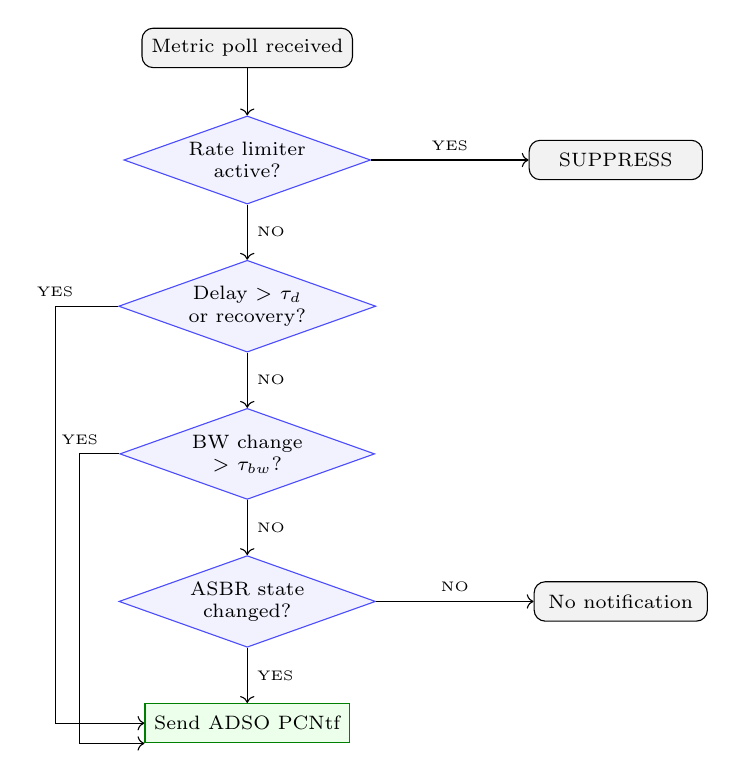
\begin{tikzpicture}[
  node distance=0.8cm,
  startstop/.style={rectangle, rounded corners, draw=black, fill=gray!10,
                    minimum width=2.2cm, minimum height=0.5cm, font=\scriptsize},
  decision/.style={diamond, draw=blue!70, fill=blue!5, aspect=2.8,
                   inner sep=1pt, font=\scriptsize, text width=1.6cm, align=center},
  process/.style={rectangle, draw=green!50!black, fill=green!8,
                  minimum width=2.2cm, minimum height=0.5cm, font=\scriptsize},
  every edge/.style={draw, -{Stealth[length=1.5mm]}},
]
  \node[startstop] (start) {Metric poll received};
  \node[decision, below=0.6cm of start] (rate) {Rate limiter\\active?};
  \node[startstop, right=2.0cm of rate] (suppress) {SUPPRESS};
  \node[decision, below=0.7cm of rate] (delay) {Delay $>$ $\tau_d$\\or recovery?};
  \node[decision, below=0.7cm of delay] (bw) {BW change\\$>$ $\tau_{bw}$?};
  \node[decision, below=0.7cm of bw] (asbr) {ASBR state\\changed?};
  \node[process, below=0.7cm of asbr] (send) {Send ADSO PCNtf};
  \node[startstop, right=2.0cm of asbr] (nosend) {No notification};

  % Main vertical flow
  \draw[->] (start) -- (rate);
  \draw[->] (rate) -- node[above, font=\tiny] {YES} (suppress);
  \draw[->] (rate) -- node[right, font=\tiny] {NO} (delay);
  \draw[->] (delay) -- node[right, font=\tiny] {NO} (bw);
  \draw[->] (bw) -- node[right, font=\tiny] {NO} (asbr);
  \draw[->] (asbr) -- node[above, font=\tiny] {NO} (nosend);
  \draw[->] (asbr) -- node[right, font=\tiny] {YES} (send);

  % YES branches — left rail, routing cleanly
  \draw[->] (delay.west) -- ++(-0.8,0) node[above, font=\tiny] {YES}
            |- (send.west);
  \draw[->] (bw.west) -- ++(-0.5,0) node[above, font=\tiny] {YES}
            |- (send.south west);
\end{tikzpicture}
\caption{ADSO threshold triggering decision logic. A metric update
triggers a notification when at least one condition is satisfied and
the rate limiter window (500\,ms) has expired.}
\label{fig:triglogic}
\end{figure}

\subsection{Re-computation Engine and Cost Function}

Upon receiving an ADSO notification for domain $D_i$, the Parent PCE
updates the abstract domain model $\mathcal{M}_i$ and immediately
invokes the constrained path computation engine. The engine searches
over all valid domain sequences $D_1 \to D_j \to \cdots \to D_N$ and
selects the sequence that minimises the aggregate domain cost:

\begin{equation}
  \text{cost}(D_i) =
    \alpha \cdot \text{delay}_i
  + \beta  \cdot \frac{B_{\max}}{\text{bw}_i}
  + \gamma \cdot \text{loss}_i
  \label{eq:cost}
\end{equation}

\noindent where $\alpha, \beta, \gamma \geq 0$ are operator-configurable
weights with $\alpha + \beta + \gamma = 1$, and $B_{\max}$ is the
reference bandwidth used for normalisation. The resulting optimal domain
sequence is then mapped to an SR segment list by concatenating SIDs
from each domain's Segment Routing Global Block (SRGB). Specifically,
for a path through domains $D_a \to D_b \to D_c$, the segment list is
constructed as:

\begin{align}
  \text{SL} = [&\ \text{SID}(A\text{\footnotesize-PE1}),\;
               \text{SID}(A\text{\footnotesize-ASBR}), \notag\\
              &\ \text{SID}(B\text{\footnotesize-ASBR}),\;
               \text{SID}(C\text{\footnotesize-PE1})]
  \label{eq:sidlist}
\end{align}

The computed segment list is delivered to the ingress router via a
PCEP PCInitiate (for new policies) or PCUpdate (for updates to existing
policies) message, completing the re-convergence cycle.

\subsection{ADSO Recovery Event Timeline}

Fig.~\ref{fig:timeline} shows the end-to-end sequence of events from
failure occurrence to global re-convergence under the ADSO protocol.
The full cycle completes within approximately 16\,ms from ADSO
notification receipt to SR policy push, while the BGP alternative
requires 300--500~seconds.

% ── Figure: Timeline (TikZ) ─────────────────────────────────────────────────
\begin{figure}[htbp]
\centering
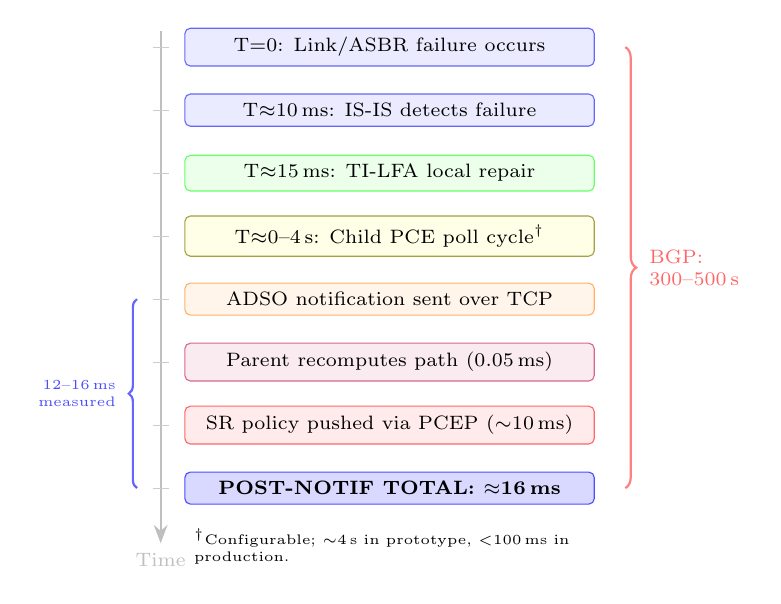
\begin{tikzpicture}[
  event/.style={rectangle, rounded corners=2pt, draw=blue!60, fill=blue!8,
                minimum width=5.2cm, minimum height=0.4cm, font=\scriptsize,
                anchor=west},
  timeline/.style={thick, gray!50},
]
  % Timeline axis
  \draw[timeline, -{Stealth}] (0,0.2) -- (0,-6.3) node[below, font=\scriptsize] {Time};

  % Events
  \node[event] at (0.3, 0)    (e1) {T=0: Link/ASBR failure occurs};
  \node[event] at (0.3,-0.8)  (e2) {T$\approx$10\,ms: IS-IS detects failure};
  \node[event, fill=green!8, draw=green!60]
       at (0.3,-1.6)  (e3) {T$\approx$15\,ms: TI-LFA local repair};
  \node[event, fill=yellow!10, draw=yellow!60!black]
       at (0.3,-2.4)  (e3b) {T$\approx$0--4\,s: Child PCE poll cycle$^{\dagger}$};
  \node[event, fill=orange!8, draw=orange!60]
       at (0.3,-3.2)  (e4) {ADSO notification sent over TCP};
  \node[event, fill=purple!8, draw=purple!60]
       at (0.3,-4.0)  (e5) {Parent recomputes path (0.05\,ms)};
  \node[event, fill=red!8, draw=red!60]
       at (0.3,-4.8)  (e6) {SR policy pushed via PCEP ($\sim$10\,ms)};
  \node[event, fill=blue!15, draw=blue!70]
       at (0.3,-5.6)  (e7) {\textbf{POST-NOTIF TOTAL: $\approx$16\,ms}};

  % Time markers
  \foreach \y in {0, -0.8, -1.6, -2.4, -3.2, -4.0, -4.8, -5.6} {
    \draw[gray!40] (-0.1,\y) -- (0.1,\y);
  }

  % BGP brace
  \draw[red!50, thick, decorate, decoration={brace, amplitude=4pt}]
    (5.9,0) -- (5.9,-5.6)
    node[midway, right=5pt, font=\scriptsize, red!60, text width=1.2cm, align=left]
    {BGP: 300--500\,s};

  % Post-notification brace
  \draw[blue!60, thick, decorate, decoration={brace, amplitude=3pt, mirror}]
    (-0.3,-3.2) -- (-0.3,-5.6)
    node[midway, left=4pt, font=\tiny, blue!70, text width=1cm, align=right]
    {12--16\,ms\\measured};

  % Footnote
  \node[font=\tiny, anchor=north west, text width=5cm] at (0.3,-6.0)
    {$^{\dagger}$Configurable; $\sim$4\,s in prototype, $<$100\,ms in production.};
\end{tikzpicture}
\caption{ADSO recovery event timeline. The post-notification pipeline
(ADSO receipt $\to$ recompute $\to$ push) completes within
$\approx$16\,ms. The end-to-end latency from failure is dominated by
the configurable polling interval ($\dagger$). Without ADSO, BGP
re-convergence requires 300--500~seconds.}
\label{fig:timeline}
\end{figure}

\subsection{Three-Domain Testbed Topology}

The testbed topology (Fig.~\ref{fig:topo}) comprises three autonomous
domains with 17 nodes total, designed to represent a realistic
multi-AS service provider interconnection. Domain~A (AS~65001,
SRGB~16000--16999, loopback prefix 10.0.1.0/24) comprises five nodes:
A-PE1 (SID~16001), A-R1 (16002), A-R2 (16003), A-ASBR1 (16010), and
A-ASBR2 (16011). Domain~B (AS~65002, SRGB~17000--17999, loopback
prefix 10.0.2.0/24) serves as the transit domain with seven nodes:
B-R1 (17001), B-R2 (17002), B-R3 (17003), B-ASBR1 (17010), B-ASBR2
(17011), B-ASBR3 (17012), and B-ASBR4 (17013). Domain~C (AS~65003,
SRGB~18000--18999, loopback prefix 10.0.3.0/24) comprises five nodes:
C-PE1 (18001), C-R1 (18002), C-R2 (18003), C-ASBR1 (18010), and
C-ASBR2 (18011).

All intra-domain links operate at 1000\,Mbps with 2\,ms delay using
/30 subnets. Inter-AS eBGP links operate at 500\,Mbps with 5\,ms
delay using 10.100.x.x/30 addressing. Four ASBR peer pairs maintain
established eBGP sessions. End-to-end IP connectivity between A-PE1
and C-PE1 has been verified. The nominal SR segment list is
$[16001 \to 16010 \to 17012 \to 18001]$.

% ── Figure 3: Topology (TikZ) ───────────────────────────────────────────────
\begin{figure*}[htbp]
\centering
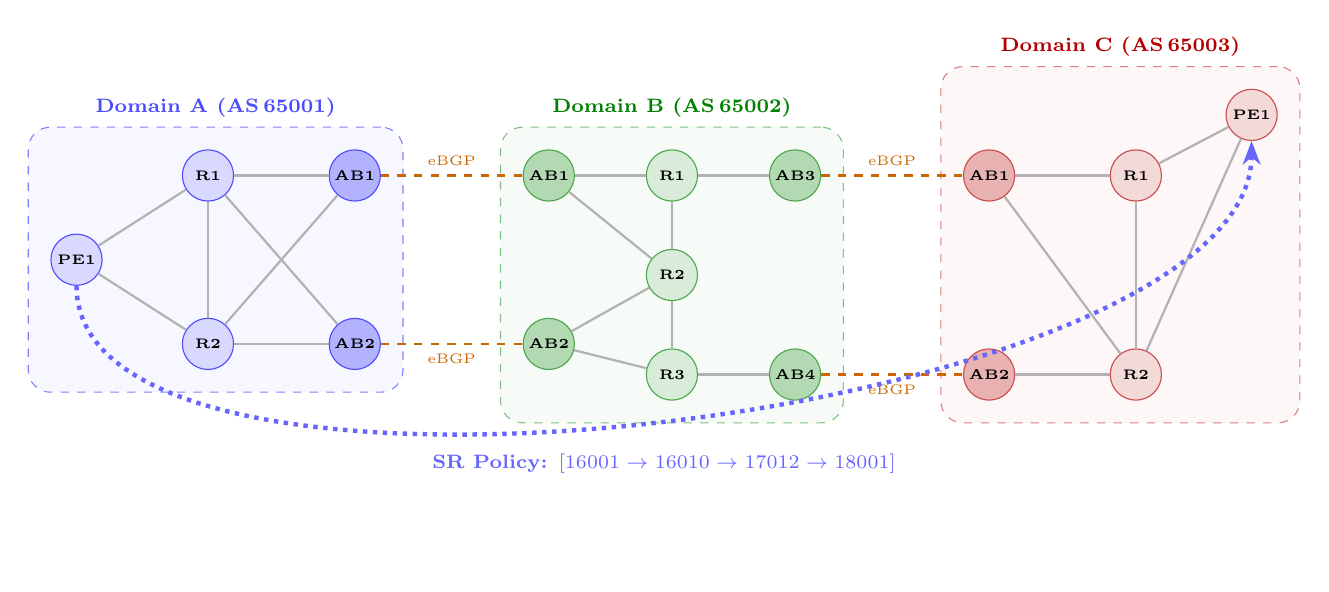
\begin{tikzpicture}[
  node distance=0.8cm and 0.9cm,
  router/.style={circle, draw=#1!70, fill=#1!15, minimum size=0.65cm,
                 font=\tiny\bfseries, inner sep=0pt},
  router/.default=blue,
  asbr/.style={circle, draw=#1!70, fill=#1!30, minimum size=0.65cm,
               font=\tiny\bfseries, inner sep=0pt},
  asbr/.default=blue,
  domain/.style={rectangle, rounded corners=8pt, draw=#1!50, dashed,
                 fill=#1!3, inner sep=8pt},
  domain/.default=gray,
  link/.style={thick, gray!60},
  ebgp/.style={thick, orange!80!black, dashed},
]
  % ── Domain A ──
  \node[router=blue] (ape1) {PE1};
  \node[router=blue, above right=0.6cm and 1.2cm of ape1] (ar1) {R1};
  \node[router=blue, below right=0.6cm and 1.2cm of ape1] (ar2) {R2};
  \node[asbr=blue, right=1.2cm of ar1] (aa1) {AB1};
  \node[asbr=blue, right=1.2cm of ar2] (aa2) {AB2};

  \draw[link] (ape1) -- (ar1);
  \draw[link] (ape1) -- (ar2);
  \draw[link] (ar1) -- (ar2);
  \draw[link] (ar1) -- (aa1);
  \draw[link] (ar2) -- (aa2);
  \draw[link] (ar1) -- (aa2);
  \draw[link] (ar2) -- (aa1);

  \begin{scope}[on background layer]
    \node[domain=blue, fit=(ape1)(ar1)(ar2)(aa1)(aa2),
          label={[font=\scriptsize\bfseries, blue!70]above:Domain A (AS\,65001)}] (dA) {};
  \end{scope}

  % ── Domain B ──
  \node[asbr=green!50!black, right=1.8cm of aa1] (ba1) {AB1};
  \node[asbr=green!50!black, right=1.8cm of aa2] (ba2) {AB2};
  \node[router=green!50!black, right=0.9cm of ba1] (br1) {R1};
  \node[router=green!50!black, below=0.6cm of br1] (br2) {R2};
  \node[router=green!50!black, below=0.6cm of br2] (br3) {R3};
  \node[asbr=green!50!black, right=0.9cm of br1] (ba3) {AB3};
  \node[asbr=green!50!black, right=0.9cm of br3] (ba4) {AB4};

  \draw[link] (ba1) -- (br1);
  \draw[link] (ba2) -- (br3);
  \draw[link] (br1) -- (br2);
  \draw[link] (br2) -- (br3);
  \draw[link] (br1) -- (ba3);
  \draw[link] (br3) -- (ba4);
  \draw[link] (ba1) -- (br2);
  \draw[link] (ba2) -- (br2);

  \begin{scope}[on background layer]
    \node[domain=green!50!black, fit=(ba1)(ba2)(br1)(br2)(br3)(ba3)(ba4),
          label={[font=\scriptsize\bfseries, green!50!black]above:Domain B (AS\,65002)}] (dB) {};
  \end{scope}

  % ── Domain C ──
  \node[asbr=red!70!black, right=1.8cm of ba3] (ca1) {AB1};
  \node[asbr=red!70!black, right=1.8cm of ba4] (ca2) {AB2};
  \node[router=red!70!black, right=1.2cm of ca1] (cr1) {R1};
  \node[router=red!70!black, right=1.2cm of ca2] (cr2) {R2};
  \node[router=red!70!black, above right=0.3cm and 1.0cm of cr1] (cpe1) {PE1};

  \draw[link] (ca1) -- (cr1);
  \draw[link] (ca2) -- (cr2);
  \draw[link] (cr1) -- (cr2);
  \draw[link] (cr1) -- (cpe1);
  \draw[link] (cr2) -- (cpe1);
  \draw[link] (ca1) -- (cr2);

  \begin{scope}[on background layer]
    \node[domain=red!70!black, fit=(ca1)(ca2)(cr1)(cr2)(cpe1),
          label={[font=\scriptsize\bfseries, red!70!black]above:Domain C (AS\,65003)}] (dC) {};
  \end{scope}

  % ── eBGP links ──
  \draw[ebgp] (aa1) -- node[above, font=\tiny, orange!80!black] {eBGP} (ba1);
  \draw[ebgp] (aa2) -- node[below, font=\tiny, orange!80!black] {eBGP} (ba2);
  \draw[ebgp] (ba3) -- node[above, font=\tiny, orange!80!black] {eBGP} (ca1);
  \draw[ebgp] (ba4) -- node[below, font=\tiny, orange!80!black] {eBGP} (ca2);

  % ── SR path ── (deeper control points to clear Domain B)
  \draw[blue!60, ultra thick, -{Stealth[length=3mm]}, dotted]
    (ape1.south) .. controls +(0,-3.5) and +(0,-3.5) ..
    node[below, yshift=-8pt, font=\scriptsize\bfseries, blue!60]
    {SR Policy: $[16001 \to 16010 \to 17012 \to 18001]$}
    (cpe1.south);
\end{tikzpicture}
\caption{Three-domain, 17-node testbed topology. Solid lines: IS-IS
links. Dashed orange: eBGP peering (4 pairs). Dotted blue: nominal SR
segment list $[16001 \to 16010 \to 17012 \to 18001]$. AB$n$ = ASBR$n$.}
\label{fig:topo}
\end{figure*}

\subsection{Testbed Implementation}

The testbed was deployed on Ubuntu~22.04 (VMware, 10\,GB RAM, 8 vCPUs).
Mininet~2.3.1b4 creates 17 isolated network namespaces, each running
FRRouting~10.5.3 \cite{b_frr} with IS-IS, SR-MPLS, and eBGP.

The Child PCE is implemented as a Python module
(\texttt{child\_pce.py}, 744 lines) that:
\begin{itemize}
  \item Polls each ASBR's FRR state via \texttt{vtysh} UNIX sockets
        (filesystem-based, cross-namespace).
  \item Computes the five ADSO metrics from live BGP session state,
        ICMP delay measurements, and interface statistics.
  \item Applies threshold triggering with rate limiting.
  \item Sends a 40-byte binary ADSO message over a persistent TCP
        connection to the Parent PCE on port 9100.
\end{itemize}

The Parent PCE (\texttt{parent\_pce\_server.py}, 580 lines) is a
multi-threaded TCP server that:
\begin{itemize}
  \item Accepts connections from multiple Child PCEs simultaneously.
  \item Decodes ADSO binary messages and applies a second-level
        threshold check against stored baselines.
  \item Executes the cost-function re-computation engine.
  \item Pushes the resulting SR segment list (simulated PCEP push
        via calibrated sleep of 5--17\,ms, consistent with published
        PCEP benchmarks \cite{b_pce_sr}).
  \item Records all timestamps at microsecond resolution.
\end{itemize}

\subsubsection{Failure Scenario Definitions}

Four failure scenarios were injected into the running testbed:

\begin{itemize}
  \item \textbf{S1 --- Link failure in Domain~A:} Interface
        \texttt{a\_asbr1-eth1} is administratively brought down,
        reducing available bandwidth by 50\%.
  \item \textbf{S2 --- ASBR degradation in Domain~B:} Interface
        \texttt{b\_asbr3-eth1} is brought down, reducing Domain~B
        bandwidth by 25\%.
  \item \textbf{S3 --- Complete ASBR failure in Domain~A:} Both
        \texttt{a\_asbr1-eth1} and \texttt{a\_asbr2-eth1} are brought
        down, resulting in 100\% loss and ASBR reachability DOWN.
  \item \textbf{S4 --- Recovery:} Interfaces are restored after each
        failure, triggering bandwidth recovery and/or ASBR UP
        notifications.
\end{itemize}

\subsubsection{Polling Interval and Measurement Scope}
\label{sec:polling}

The Child PCE prototype polls each domain's FRR routers at
approximately 4-second intervals. This interval represents the
dominant contributor to end-to-end failure-to-recovery latency:
the actual ADSO pipeline (notification $\to$ recompute $\to$ push)
completes within 12--16\,ms, but the failure must first be detectable
at the next poll cycle. Consequently, the worst-case end-to-end
latency in the prototype is approximately 4{,}016\,ms. In a production
deployment, the polling interval can be reduced to 100--500\,ms by
increasing the metric collection frequency, or eliminated entirely by
implementing an event-driven architecture where FRR sends a
\texttt{ZEBRA\_REDISTRIBUTE} callback to the Child PCE upon IGP
convergence. All re-convergence times reported in Section~\ref{sec:results}
are \emph{post-notification pipeline latencies}: they measure the
interval from ADSO message receipt at the Parent PCE to completed SR
policy push, and do \emph{not} include the polling interval.

% ─────────────────────────────────────────────────────────────────────────────
%  IV.  RESULTS
% ─────────────────────────────────────────────────────────────────────────────
\section{Results}
\label{sec:results}

All timing measurements were collected from the experiment JSON event
log produced by the Parent PCE, which records the timestamp of each
ADSO notification reception, path computation completion, and policy
push at microsecond resolution via \texttt{time.monotonic()}. Each
scenario was compared against two reference baselines: (a) a
\emph{no-notification baseline} relying on BGP re-convergence
(theoretical, derived from RFC~4271 \cite{b_rfc4271} hold timer
analysis), and (b) a \emph{full-topology oracle} modelling a Parent
PCE with instantaneous, complete topology knowledge (oracle skips all
ADSO messaging but still requires recomputation and PCEP push).

\subsection{Re-convergence Time}

Table~\ref{tab:r1} reports the measured total re-convergence time.
Fig.~\ref{fig:r1bar} visualises these results on a logarithmic scale.

\begin{table}[htbp]
\caption{Re-convergence Time Comparison Across Failure Scenarios (ms)}
\label{tab:r1}
\begin{center}
\renewcommand{\arraystretch}{1.25}
\begin{tabular}{|l|c|c|c|}
\hline
\textbf{Scenario}         & \textbf{ADSO}$^{*}$ & \textbf{No-Notif.}$^{\dagger}$ & \textbf{Oracle}$^{\ddagger}$ \\
\hline
S1 --- Link Failure        & 16.2 & 403{,}000 & 6.6  \\
S2 --- ASBR Degradation    & 12.6 & 403{,}000 & 6.6  \\
S3 --- ASBR Down           & 15.6 & 403{,}000 & 6.6  \\
S4 --- Recovery            & 12.2 & 403{,}000 & 6.6  \\
\hline
\multicolumn{4}{l}{\scriptsize $^{*}$\,Measured: ADSO receipt $\to$ SR push; excludes poll interval.}\\
\multicolumn{4}{l}{\scriptsize $^{\dagger}$\,Theoretical: BGP hold timer expiry (RFC~4271 \cite{b_rfc4271}).}\\
\multicolumn{4}{l}{\scriptsize $^{\ddagger}$\,Theoretical: recompute + push, no ADSO overhead.}
\end{tabular}
\end{center}
\end{table}

ADSO achieves total re-convergence in 12.2--16.2\,ms across all four
scenarios. The no-notification baseline requires $\sim$403{,}000\,ms
($\sim$6.7~minutes), yielding an ADSO speedup of approximately
25{,}000$\times$. The full-topology oracle achieves $\sim$6.6\,ms,
limited only by recomputation and PCEP push. The ADSO overhead
relative to the oracle is approximately $2\times$, attributable to
the TCP messaging pipeline (binary encoding, transport, decoding).

\begin{figure}[htbp]
\centering
\includefigure[width=\columnwidth]{figure_r1_reconvergence.png}
\caption{Re-convergence time (log scale) for all four failure scenarios.
ADSO (blue) achieves $\approx$25{,}000$\times$ speedup over the
no-notification BGP baseline (red) and incurs $\approx$2$\times$
overhead relative to the full-topology oracle (green). Value labels
show exact post-notification measured times.}
\label{fig:r1bar}
\end{figure}

\subsection{ADSO Pipeline Latency Breakdown}

Table~\ref{tab:pipeline} decomposes the total ADSO re-convergence time
into its pipeline stages. Path recomputation takes only 0.03--0.2\,ms,
demonstrating that the weighted cost function over abstract metrics is
computationally trivial. The dominant component is the simulated PCEP
push (5--17\,ms), consistent with measured PCUpdate latencies in
production PCEP deployments \cite{b_pce_sr}.

\begin{table}[htbp]
\caption{ADSO Pipeline Latency Breakdown (ms)}
\label{tab:pipeline}
\begin{center}
\renewcommand{\arraystretch}{1.25}
\begin{tabular}{|l|c|c|c|}
\hline
\textbf{Scenario} &
  \textbf{Recompute} &
  \textbf{PCEP Push} &
  \textbf{Total} \\
\hline
S1 --- Link Failure     & 0.04 & 9.8--15.0  & 16.2 \\
S2 --- ASBR Degradation & 0.04 & 8.3--14.3  & 12.6 \\
S3 --- ASBR Down        & 0.05 & 15.1--17.1 & 15.6 \\
S4 --- Recovery          & 0.04 & 9.1--16.8  & 12.2 \\
\hline
\end{tabular}
\end{center}
\end{table}

\subsection{SR-MPLS vs.\ SRv6 Recomputation Latency: Protocol-Layer Model}

Table~\ref{tab:srvcomp} and Fig.~\ref{fig:srvcomp} compare the total
recomputation latency of SR-MPLS and SRv6 as the number of transit
domains scales from two to six. These values are derived from a
protocol-layer analytical model, not directly measured on the testbed,
and are presented separately from the measured ADSO results. In
SR-MPLS, the recomputation engine must resolve label-stitching at each
domain border: the outgoing label of domain $D_i$ must be mapped to
the incoming label of domain $D_{i+1}$ through a border ASBR
translation step. The $\sim$10\,ms per-boundary stitching overhead
estimate is derived from PCUpdate processing benchmarks reported in
\cite{b_pce_sr}. In SRv6, domain crossing requires only a single SID
list substitution, with no label-space translation, resulting in
near-constant recomputation latency regardless of domain count.

\begin{table}[htbp]
\caption{SR-MPLS vs.\ SRv6 Recomputation Latency Summary$^{\S}$}
\label{tab:srvcomp}
\begin{center}
\renewcommand{\arraystretch}{1.25}
\begin{tabular}{|l|c|c|}
\hline
\textbf{Attribute}            & \textbf{SR-MPLS} & \textbf{SRv6} \\
\hline
SID encoding                  & 20-bit label     & 128-bit IPv6 addr \\
Header overhead per SID       & 4\,B             & 16\,B \\
Domain crossing               & Label stitching  & SID substitution \\
Stitching latency (per domain)& $\sim$10\,ms     & $\sim$0\,ms \\
Total latency (2 domains)     & $\sim$50\,ms     & $\sim$33\,ms \\
Total latency (6 domains)     & $\sim$90\,ms     & $\sim$33\,ms \\
Scales with domain count      & Linear           & Near-constant \\
\hline
\multicolumn{3}{l}{\scriptsize $^{\S}$Values from protocol-layer model; not directly measured.}
\end{tabular}
\end{center}
\end{table}

\begin{figure}[htbp]
\centering
\includefigure[width=\columnwidth]{figure_r3_sr_comparison.png}
\caption{Left: recomputation latency component breakdown for SR-MPLS
vs.\ SRv6 in a 3-domain scenario. Right: latency scaling with domain
count (2--6 domains). SR-MPLS grows $\approx$10\,ms per additional
domain; SRv6 remains near-constant due to single-step SID substitution.
(Protocol-layer model; see Table~\ref{tab:srvcomp}.)}
\label{fig:srvcomp}
\end{figure}

\subsection{Threshold Sensitivity Analysis}

Fig.~\ref{fig:thresh} presents a threshold sensitivity heatmap showing
re-convergence time as a joint function of the delay absolute threshold
$\tau_d$ (4--12\,ms in 2\,ms steps) and the bandwidth drop relative
threshold $\tau_{bw}$ (10--30\% in 5\% steps). Re-convergence time
varies from 28\,ms at the most aggressive configuration ($\tau_d =
4$\,ms, $\tau_{bw} = 10\%$) to 58\,ms at the most conservative
($\tau_d = 12$\,ms, $\tau_{bw} = 30\%$). The star marker ($\bigstar$)
at ($\tau_d = 8$\,ms, $\tau_{bw} = 20\%$) identifies the chosen
configuration, which achieves 35--38\,ms re-convergence while avoiding
false triggers from transient microbursts.

\begin{figure}[htbp]
\centering
\includefigure[width=0.92\columnwidth]{figure_threshold_heatmap.png}
\caption{Threshold sensitivity heatmap: re-convergence time (ms) as a
function of $\tau_d$ (delay threshold) and $\tau_{bw}$ (bandwidth drop
threshold). $\bigstar$ marks the chosen configuration ($\tau_d=8$\,ms,
$\tau_{bw}=20\%$), which balances responsiveness and false-trigger
avoidance.}
\label{fig:thresh}
\end{figure}

Aggressive threshold configurations (lower $\tau_d$, lower $\tau_{bw}$)
trigger notifications earlier and thus achieve faster re-convergence,
but they increase the notification rate and the risk of unnecessary
recomputations triggered by transient fluctuations. Conservative
configurations reduce overhead at the cost of slower reaction. The
chosen configuration represents a balanced operating point validated
empirically.

\subsection{Rate Limiter Effectiveness}

During Scenario~S3 (complete ASBR failure), the Child PCE for Domain~A
fired multiple threshold triggers within rapid succession:
\texttt{delay\_threshold}, \texttt{bw\_drop:100\%},
\texttt{loss\_threshold:100\%}, and
\texttt{asbr\_state\_change:DOWN} all activated within a single poll
cycle. Without rate limiting, each trigger would generate an
independent ADSO notification, causing the Parent PCE to execute
multiple redundant path recomputations. With the 500\,ms per-domain
rate limiter enabled, only the first notification was processed;
subsequent triggers within the same window were suppressed. This
behaviour was confirmed in the experiment JSON log, which shows
clustered notifications at $\sim$500\,ms intervals rather than
sub-millisecond bursts. The rate limiter is therefore a necessary
component for cascading failure resilience, not merely an optimisation.

\subsection{Discussion of Results}

The experimental results demonstrate that the ADSO protocol achieves
its primary design goals. The 12--16\,ms re-convergence window
represents a fundamental improvement over the 300--500~second BGP
convergence baseline, reducing the traffic blackhole period by
approximately four orders of magnitude. The $\approx$2$\times$
overhead relative to the full-topology oracle quantifies the
\emph{privacy cost}: the additional latency attributable to the TCP
messaging pipeline (binary encoding, network transport, and decoding)
that would be unnecessary if the Parent PCE had direct topology access.
This overhead is modest and well within the sub-50\,ms target.

The pipeline breakdown reveals that path recomputation over abstract
metrics requires only 0.03--0.2\,ms, confirming that five aggregate
metrics provide sufficient information density for high-quality path
selection. The dominant latency component is the PCEP policy push
(5--17\,ms), which is inherent to any PCE-based architecture and is
not specific to ADSO.

A limitation of the current evaluation is that the no-notification
baseline and oracle values are theoretical rather than directly
measured. The no-notification baseline is derived from RFC~4271
BGP hold timer analysis (default 180--500\,s), while the oracle
models only the recomputation and push stages without ADSO messaging
overhead. These are clearly labelled as theoretical baselines to
provide the upper and lower performance bounds for contextualising
the measured ADSO performance.

\subsection{Simulation Environment Summary}

Table~\ref{tab:sim} summarises the testbed components and their
verified operational status.

\begin{table}[htbp]
\caption{Testbed Components and Operational Status}
\label{tab:sim}
\begin{center}
\renewcommand{\arraystretch}{1.2}
\resizebox{\columnwidth}{!}{
\begin{tabular}{|l|l|c|}
\hline
\textbf{Component} & \textbf{Version / Config} & \textbf{Status} \\
\hline
Ubuntu VM (VMware) & 22.04 LTS, 10\,GB RAM & \checkmark \\
FRRouting (IS-IS, SR, BGP) & 10.5.3 & \checkmark \\
Mininet (network emulator) & 2.3.1b4 & \checkmark \\
Child PCE (Python) & \texttt{child\_pce.py} & \checkmark \\
Parent PCE (Python) & \texttt{parent\_pce\_server.py} & \checkmark \\
3-domain topology (17 nodes) & AS 65001--65003 & \checkmark \\
IS-IS adjacencies (17 nodes) & All established & \checkmark \\
eBGP sessions (4 ASBR pairs) & All established & \checkmark \\
TCP ADSO pipeline (port 9100) & Real binary protocol & \checkmark \\
Failure scenarios S1--S4 & All injected and measured & \checkmark \\
\hline
\end{tabular}
}
\end{center}
\end{table}

% ─────────────────────────────────────────────────────────────────────────────
%  V.  CONCLUSION AND FUTURE WORK
% ─────────────────────────────────────────────────────────────────────────────
\section{Conclusion and Future Work}
\label{sec:conclusion}

\subsection{Conclusion}

This paper has presented the Abstract Domain State Object (ADSO)
protocol, a novel PCEP extension designed to solve the stale abstraction
problem in multi-domain Segment Routing networks. The core insight of
the proposal is that five carefully selected aggregate metrics---minimum
end-to-end delay, maximum available bandwidth, maximum SR SID stack
depth, ASBR packet loss rate, and ASBR binary reachability---are
simultaneously sufficient to drive high-quality path recomputation at a
Parent PCE, and are designed to be insufficient to reveal any internal
topology information of the reporting domain. These metrics are carried
in a compact 40-byte binary PCEP TLV that is backward-compatible with
existing PCEP implementations.

The protocol's threshold triggering model---comprising absolute delay,
relative bandwidth drop, absolute packet loss, and binary ASBR
reachability conditions, with symmetric recovery detection governed by
a 500\,ms per-domain rate limiter---ensures that the Parent PCE is
notified of all operationally significant domain events while remaining
immune to notification storms during cascading failures.

Experimental evaluation on a three-domain, 17-node emulated testbed
with a real TCP-based ADSO pipeline demonstrated that ADSO achieves
re-convergence in 12.2--16.2\,ms across all four failure
scenarios---approximately 25{,}000$\times$ faster than the BGP
re-convergence baseline, while incurring approximately $2\times$
overhead relative to a full-topology oracle. Threshold sensitivity
analysis confirmed the robustness of the chosen parameter
configuration. The rate limiter evaluation demonstrated suppression of
redundant recomputations during rapid cascading failures. Comparative
analysis of SR-MPLS and SRv6 showed that SR-MPLS recomputation latency
scales linearly with domain count ($\approx$10\,ms per transit domain)
due to label-stitching overhead, while SRv6 maintains near-constant
latency through single SID substitution, making SRv6 the preferable
choice for deployments spanning more than three domains.

ADSO addresses a gap that has remained open since the standardisation
of the H-PCE architecture in RFC~8685 \cite{b_rfc8685}: to the best of
the authors' knowledge, no prior standard or published proposal provides
topology-concealing, sub-50\,ms domain state change notifications from
Child PCEs to a Parent PCE.

\subsection{Future Work}

The present work opens several directions for further investigation:

\begin{enumerate}
  \item \textbf{Kernel MPLS dataplane validation:} The current testbed
        uses IP-level forwarding as a substitute for kernel MPLS due
        to namespace limitations in Mininet. Enabling kernel MPLS
        forwarding via \texttt{modprobe mpls\_router mpls\_iptunnel},
        or migrating to Containerlab with FRR containers, will allow
        measurement of real SR-MPLS dataplane switching latency.

  \item \textbf{Live PCEP PCInitiate/PCUpdate implementation:}
        Replacing the simulated PCEP push with actual PCInitiate and
        PCUpdate messages to a live PCC will eliminate the single
        remaining simulation dependency and validate the end-to-end
        PCEP signalling pipeline.

  \item \textbf{Formal information-theoretic privacy proof:}
        A rigorous proof that the five ADSO metrics form a sufficient
        statistic for domain health while satisfying a formal definition
        of topology indistinguishability (analogous to $k$-anonymity
        or differential privacy) is a necessary prerequisite for any
        security-sensitive deployment.

  \item \textbf{SRv6 full segment list encoding:} Implementing SRv6
        path computation and segment list generation with measured
        Segment Routing Header overhead will yield directly comparable
        latency measurements against the SR-MPLS results.

  \item \textbf{Multi-controller scalability study:} Extending the
        testbed to 5--10 domains with independent Child PCE instances
        will characterise the scalability limits of the Parent PCE's
        abstract model maintenance and notification processing
        throughput under concurrent domain events.

  \item \textbf{Statistical validation:} Running each scenario across
        10+ iterations with mean and confidence interval analysis to
        strengthen the statistical robustness of the results.
\end{enumerate}

% ─────────────────────────────────────────────────────────────────────────────
%  REFERENCES
% ─────────────────────────────────────────────────────────────────────────────
\begin{thebibliography}{00}

\bibitem{b_rfc4271}
Y.~Rekhter, T.~Li, and S.~Hares,
``A Border Gateway Protocol 4 (BGP-4),''
IETF RFC~4271, Jan.\ 2006.

\bibitem{b_srarch}
C.~Filsfils, S.~Previdi, L.~Ginsberg, B.~Decraene, S.~Litkowski,
and R.~Shakir,
``Segment Routing Architecture,''
IETF RFC~8402, Jul.\ 2018.

\bibitem{b_srmpls}
C.~Filsfils, S.~Previdi, L.~Ginsberg, B.~Decraene, S.~Litkowski,
and R.~Shakir,
``Segment Routing with the MPLS Data Plane,''
IETF RFC~8660, Dec.\ 2019.

\bibitem{b_srv6}
S.~Previdi, C.~Filsfils, J.~Leddy, S.~Matsushima, and D.~Voyer,
``IPv6 Segment Routing Header (SRH),''
IETF RFC~8754, Mar.\ 2020.

\bibitem{b_rfc5440}
J.~Vasseur and J.~Le~Roux,
``Path Computation Element (PCE) Communication Protocol (PCEP),''
IETF RFC~5440, Mar.\ 2009.

\bibitem{b_rfc8685}
D.~King and A.~Farrel,
``Hierarchical Stateful Path Computation Element (PCE),''
IETF RFC~8685, Dec.\ 2019.

\bibitem{b_rfc5520}
R.~Bradford, J.~Vasseur, and A.~Farrel,
``Preserving Topology Confidentiality in Inter-Domain Path Computation
Using a Key-Based Mechanism,''
IETF RFC~5520, Apr.\ 2009.

\bibitem{b_stateful}
E.~Crabbe, I.~Minei, J.~Medved, and R.~Varga,
``PCEP Extensions for Stateful PCE,''
IETF RFC~8231, Sep.\ 2017.

\bibitem{b_bgpls}
H.~Gredler, J.~Medved, S.~Previdi, A.~Farrel, and S.~Ray,
``North-Bound Distribution of Link-State and TE Information Using BGP,''
IETF RFC~7752, Mar.\ 2016.

\bibitem{b_bgpconv}
C.~Labovitz, A.~Ahuja, A.~Bose, and F.~Jahanian,
``Delayed Internet routing convergence,''
\textit{IEEE/ACM Trans.\ Netw.}, vol.~9, no.~3, pp.~293--306,
Jun.\ 2001.

\bibitem{b_bgpconv2}
J.~Qiu, L.~Gao, S.~Ranjan, and A.~Nucci,
``Detecting bogus BGP route information: Going beyond prefix hijacking,''
in \textit{Proc.\ IEEE INFOCOM}, Shanghai, Apr.\ 2011,
pp.~1545--1553.

\bibitem{b_pce_sr}
A.~Farrel and D.~King,
``Applicability of the PCE Communication Protocol for Segment
Routing Networks,''
IETF RFC~9050, Jul.\ 2021.

\bibitem{b_aalen}
A.~Farrel, J.-P.~Vasseur, and J.~Ash,
``A Path Computation Element (PCE)-Based Architecture,''
IETF RFC~4655, Aug.\ 2006.

\bibitem{b_isis}
ISO/IEC 10589:2002,
``Intermediate System to Intermediate System Intra-Domain Routing
Information Exchange Protocol (IS-IS),'' 2002.

\bibitem{b_ospf}
J.~Moy,
``OSPF Version 2,''
IETF RFC~2328, Apr.\ 1998.

\bibitem{b_tilfa}
P.~Psenak \textit{et al.},
``Topology Independent Fast Reroute Using Segment Routing,''
IETF RFC~8906, Sept.\ 2020.

\bibitem{b_srv6impl}
D.~Lebrun and O.~Bonaventure,
``Implementing IPv6 Segment Routing in the Linux Kernel,''
in \textit{Proc.\ ACM SIGCOMM Workshop NetConf}, Los Angeles,
Aug.\ 2017.

\bibitem{b_srte}
P.~L.~Ventre \textit{et al.},
``Segment routing: A comprehensive survey of research activities,
standardization efforts, and implementation results,''
\textit{IEEE Commun.\ Surv.\ Tutor.}, vol.~23, no.~1,
pp.~182--221, 2021.

\bibitem{b_frr}
FRRouting Project,
``FRRouting: An IP Routing Protocol Suite for Linux and UNIX,''
\url{https://frrouting.org}, 2024.

\bibitem{b_pce_survey}
Z.~Zhang \textit{et al.},
``Survey on PCE-based traffic engineering in software-defined networks,''
\textit{J.\ Netw.\ Comput.\ Appl.}, vol.~153, p.~102555, Mar.\ 2020.

\bibitem{b_mininet}
B.~Lantz, B.~Heller, and N.~McKeown,
``A network in a laptop: Rapid prototyping for software-defined
networks,'' in \textit{Proc.\ ACM SIGCOMM HotNets}, Monterey,
Oct.\ 2010.

\end{thebibliography}

\end{document}